\documentclass[paper=letter, fontsize=11pt]{scrartcl} % Letter paper and 11pt font size

\usepackage{amstext, amsmath, amssymb, graphicx}
\usepackage[T1]{fontenc} % Use 8-bit encoding that has 256 glyphs
\usepackage[english]{babel} % English language/hyphenation
\usepackage{amsmath,amsfonts,amsthm} % Math packages

\usepackage{fancyhdr} % Custom headers and footers
\pagestyle{fancyplain} % Makes all pages in the document conform to the custom headers and footers
\fancyhead{} % No page header
\fancyfoot[L]{} % Empty left footer
\fancyfoot[C]{} % Empty center footer
\fancyfoot[R]{\thepage} % Page numbering for right footer
\renewcommand{\headrulewidth}{0pt} % Remove header underlines
\renewcommand{\footrulewidth}{0pt} % Remove footer underlines
\setlength{\headheight}{13.6pt} % Customize the height of the header
\setlength\parindent{0pt} % Remove all indentation from paragraps.


%----------------------------------------------------------------------------------------
%	TITLE SECTION
%----------------------------------------------------------------------------------------

\newcommand{\horrule}[1]{\rule{\linewidth}{#1}} % Create horizontal rule command with 1 argument of height

\title{	
\normalfont \normalsize 
\textsc{San Francisco State University} \\ [25pt]
\horrule{0.5pt} \\[0.4cm] % Thin top horizontal rule
\huge MATH 490 Assignment 3 \\ % The assignment title
\horrule{2pt} \\[0.5cm] % Thick bottom horizontal rule
}

\author{Omar Sandoval}

\date{\normalsize\today}

\begin{document}

\maketitle

%----------------------------------------------------------------------------------------
%	PROBLEM 2.18
%----------------------------------------------------------------------------------------
\textbf{2.18}	Table 2.13 shows data from the 2002 General Social Survey cross classifying
a person's perceived happiness with their family income. The table displays the observed
and expected cell counts and the standardized residuals for testing independence. \\

\textbf{a.}	Show how to obtain the estimated expected cell count of 35.8 for the first cell.
\\

\textbf{b.} For testing independence, $X^2 = 73.4$. Report the $df$ value and the P-value, 
and interpret. \\

\textbf{c.} Interpret the standardized residuals in the corner cells having counts 21 and 
83. \\

\textbf{d.} Interpret the standardized residuals in the corner cells having counts 110 and
94. \\

\begin{center}
	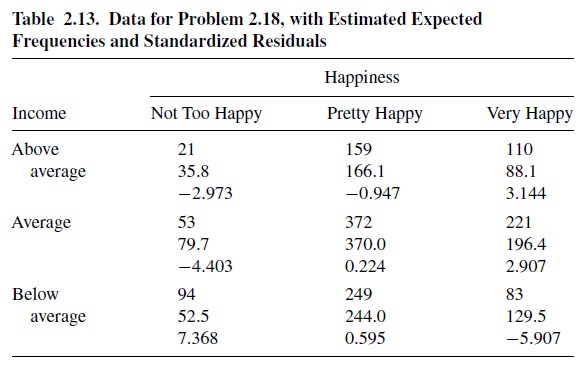
\includegraphics[scale=.80]{table213.png}
\end{center}

%----------------------------------------------------------------------------------------
%	PROBLEM 2.21
%----------------------------------------------------------------------------------------
\textbf{2.21} Each subject in a sample of 100 men and 100 women is asked to indicate which
of the following factors (one or more) are responsible for increases in teenage crime. A,
the increasing gap in income between the rich and poor; B, the increase in the percentage
of single-parent families; C, insufficient time spent by parents with their children. A 
cross classification of the responses by gender is \\

\begin{center}
	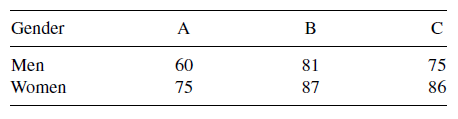
\includegraphics[scale=.80]{contTable221.png}
\end{center}

\textbf{a.} Is it valid to apply the chi-squared test of independence to this $2 \times 3$
table? Explain. \\

\textbf{b.} Explain how this table actually provides information needed to cross-classify
gender with each of three variables. Construct the contingency table relating gender to
opinion about whether factor A is responsible for increases in teenage crime. \\

%----------------------------------------------------------------------------------------
%	PROBLEM 2.22
%----------------------------------------------------------------------------------------
\textbf{2.22} Table 2.15 classifies a sample of psychiatric patients by their diagnosis
and by whether their treatment prescribed drugs. \\

\textbf{a.} Conduct a test of independence, and interpret the P-value. \\

\textbf{b.} Obtain standardized residuals, and interpret. \\

\begin{center}
	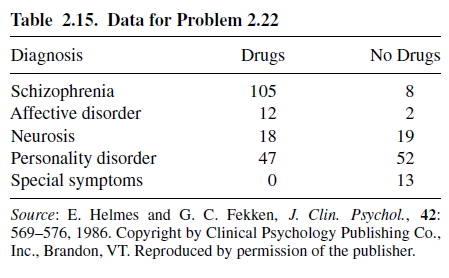
\includegraphics[scale=.80]{table215.png}
\end{center}

\textbf{c.} Partition chi-squared into three components to describe differences and
similarities among the diagnoses, by comparing (i) the first rows, (ii) the third and
fourth rows, (iii) the last row to the first and second rows combined and the third
and fourth rows combined. \\

%----------------------------------------------------------------------------------------
%	PROBLEM 2.30
%----------------------------------------------------------------------------------------
\textbf{2.30} Table 2.17 contains results of a study comparing radiation therapy with
surgery in treating cancer of the larynx. User Fisher's exact test to test $H_0: \theta =
1$ against $H_a: \theta > 1$. Interpret results. \\

\begin{center}
	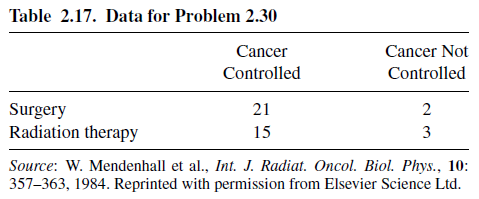
\includegraphics[scale=.80]{table217.png}
\end{center}

%----------------------------------------------------------------------------------------
%	PROBLEM 2.33
%----------------------------------------------------------------------------------------
\textbf{2.33} In murder trials in 20 Florida counties during 1976 and 1977, the death penalty was given in 19 out of 151 cases in which a white killed a white, in 0 out of 9 cases in 
which a white killed a black, in 11 out of 63 cases in which a black killed a white, and 
in 6 out of 103 cases in which a black killed a black. (M. Radelet, \textit{Am. Sociol. 
Rev.,} \textbf{46}: 918-927, 1981). \\

\textbf{a.} Exhibit the data as a three-way contingency table. \\

\textbf{b.} Construct the partial tables needed to study the conditional association 
between defendant's race and the death penalty verdict. Find and interpret the sample
conditional odds ratios, adding 0.5 to each cell to reduce the impact of the 0 cell count.
\\

\textbf{c.} Compute and interpret the sample maginal odds ratio between defendant's race
and the death penalty verdict. Do these data exhibit Simpson's paradox? Explain. \\

%----------------------------------------------------------------------------------------
%	PROBLEM 2.38
%----------------------------------------------------------------------------------------
\textbf{2.38} For three-way contingency tables: \\

\textbf{a.} When any pair of variables is conditionally independent, explain why there is
homogeneous association. \\

\textbf{b.} When there is not homogeneous association, explain why no pair of variables can
be conditionally independent. \\

\end{document}
